\chapter{Liên thông mạnh (Strong connectivity)}

\index{strongly connected graph}

Trong một đồ thị có hướng,
các cạnh chỉ có thể được duyệt theo một hướng,
vì vậy ngay cả khi đồ thị là liên thông,
điều này không đảm bảo rằng sẽ có
một đường đi từ một nút đến một nút khác.
Vì lý do này, việc định nghĩa một khái niệm mới
đòi hỏi nhiều hơn tính liên thông là có ý nghĩa.

Một đồ thị được gọi là \key{liên thông mạnh (strongly connected)}
nếu có một đường đi từ bất kỳ nút nào đến tất cả
các nút khác trong đồ thị.
Ví dụ, trong hình sau,
đồ thị bên trái là liên thông mạnh
trong khi đồ thị bên phải thì không.

\begin{center}
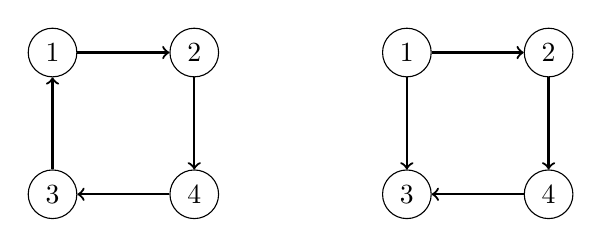
\begin{tikzpicture}[scale=0.9]
\node[draw, circle] (1) at (1,1) {$1$};
\node[draw, circle] (2) at (3,1) {$2$};
\node[draw, circle] (3) at (1,-1) {$3$};
\node[draw, circle] (4) at (3,-1) {$4$};

\path[draw,thick,->] (1) -- (2);
\path[draw,thick,->] (2) -- (4);
\path[draw,thick,->] (4) -- (3);
\path[draw,thick,->] (3) -- (1);

\node[draw, circle] (1b) at (6,1) {$1$};
\node[draw, circle] (2b) at (8,1) {$2$};
\node[draw, circle] (3b) at (6,-1) {$3$};
\node[draw, circle] (4b) at (8,-1) {$4$};

\path[draw,thick,->] (1b) -- (2b);
\path[draw,thick,->] (2b) -- (4b);
\path[draw,thick,->] (4b) -- (3b);
\path[draw,thick,->] (1b) -- (3b);
\end{tikzpicture}
\end{center}

Đồ thị bên phải không liên thông mạnh
bởi vì, ví dụ, không có đường đi
từ nút 2 đến nút 1.

\index{strongly connected component}
\index{component graph}

Các \key{thành phần liên thông mạnh (strongly connected components)}
của một đồ thị chia đồ thị thành các phần liên thông mạnh
lớn nhất có thể.
Các thành phần liên thông mạnh tạo thành một
\key{đồ thị thành phần (component graph)} không có chu trình, đại diện cho
cấu trúc sâu của đồ thị ban đầu.

Ví dụ, đối với đồ thị
\begin{center}
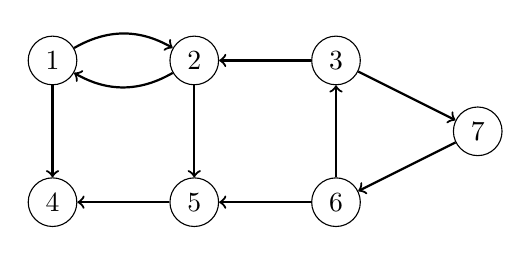
\begin{tikzpicture}[scale=0.9,label distance=-2mm]
\node[draw, circle] (1) at (-1,1) {$7$};
\node[draw, circle] (2) at (-3,2) {$3$};
\node[draw, circle] (4) at (-5,2) {$2$};
\node[draw, circle] (6) at (-7,2) {$1$};
\node[draw, circle] (3) at (-3,0) {$6$};
\node[draw, circle] (5) at (-5,0) {$5$};
\node[draw, circle] (7) at (-7,0) {$4$};

\path[draw,thick,->] (2) -- (1);
\path[draw,thick,->] (1) -- (3);
\path[draw,thick,->] (3) -- (2);
\path[draw,thick,->] (2) -- (4);
\path[draw,thick,->] (3) -- (5);
\path[draw,thick,->] (4) edge [bend left] (6);
\path[draw,thick,->] (6) edge [bend left] (4);
\path[draw,thick,->] (4) -- (5);
\path[draw,thick,->] (5) -- (7);
\path[draw,thick,->] (6) -- (7);
\end{tikzpicture}
\end{center}
các thành phần liên thông mạnh như sau:
\begin{center}
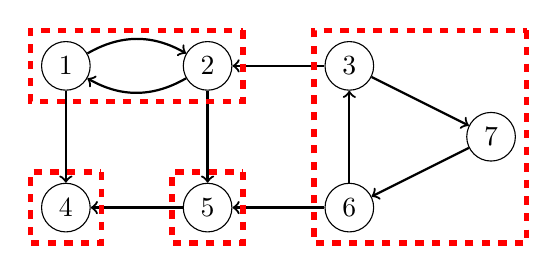
\begin{tikzpicture}[scale=0.9]
\node[draw, circle] (1) at (-1,1) {$7$};
\node[draw, circle] (2) at (-3,2) {$3$};
\node[draw, circle] (4) at (-5,2) {$2$};
\node[draw, circle] (6) at (-7,2) {$1$};
\node[draw, circle] (3) at (-3,0) {$6$};
\node[draw, circle] (5) at (-5,0) {$5$};
\node[draw, circle] (7) at (-7,0) {$4$};

\path[draw,thick,->] (2) -- (1);
\path[draw,thick,->] (1) -- (3);
\path[draw,thick,->] (3) -- (2);
\path[draw,thick,->] (2) -- (4);
\path[draw,thick,->] (3) -- (5);
\path[draw,thick,->] (4) edge [bend left] (6);
\path[draw,thick,->] (6) edge [bend left] (4);
\path[draw,thick,->] (4) -- (5);
\path[draw,thick,->] (5) -- (7);
\path[draw,thick,->] (6) -- (7);

\draw [red,thick,dashed,line width=2pt] (-0.5,2.5) rectangle (-3.5,-0.5);
\draw [red,thick,dashed,line width=2pt] (-4.5,2.5) rectangle (-7.5,1.5);
\draw [red,thick,dashed,line width=2pt] (-4.5,0.5) rectangle (-5.5,-0.5);
\draw [red,thick,dashed,line width=2pt] (-6.5,0.5) rectangle (-7.5,-0.5);
\end{tikzpicture}
\end{center}
Đồ thị thành phần tương ứng như sau:
\begin{center}
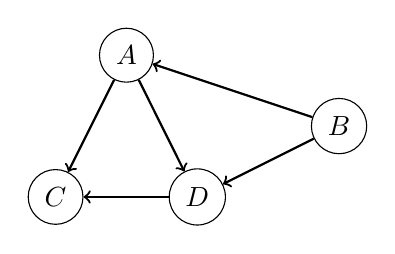
\begin{tikzpicture}[scale=0.9]
\node[draw, circle] (1) at (-3,1) {$B$};
\node[draw, circle] (2) at (-6,2) {$A$};
\node[draw, circle] (3) at (-5,0) {$D$};
\node[draw, circle] (4) at (-7,0) {$C$};

\path[draw,thick,->] (1) -- (2);
\path[draw,thick,->] (1) -- (3);
\path[draw,thick,->] (2) -- (3);
\path[draw,thick,->] (2) -- (4);
\path[draw,thick,->] (3) -- (4);
\end{tikzpicture}
\end{center}
Các thành phần là $A=\{1,2\}$,
$B=\{3,6,7\}$, $C=\{4\}$ và $D=\{5\}$.

Một đồ thị thành phần là một đồ thị có hướng, không chu trình,
vì vậy nó dễ xử lý hơn đồ thị ban đầu.
Vì đồ thị không chứa chu trình,
chúng ta luôn có thể xây dựng một sắp xếp tô pô và
sử dụng các kỹ thuật quy hoạch động như những kỹ thuật
đã được trình bày trong Chương 16.

\section{Thuật toán Kosaraju}

\index{Kosaraju's algorithm}

\key{Thuật toán Kosaraju (Kosaraju's algorithm)}\footnote{Theo \cite{aho83},
S. R. Kosaraju đã phát minh ra thuật toán này vào năm 1978
nhưng không công bố nó. Năm 1981, thuật toán tương tự đã được tái khám phá
và công bố bởi M. Sharir \cite{sha81}.} là một phương pháp hiệu quả
để tìm các thành phần liên thông mạnh
của một đồ thị có hướng.
Thuật toán thực hiện hai lần tìm kiếm theo chiều sâu:
lần tìm kiếm thứ nhất xây dựng một danh sách các nút
theo cấu trúc của đồ thị,
và lần tìm kiếm thứ hai hình thành các thành phần liên thông mạnh.

\subsubsection{Tìm kiếm 1}

Giai đoạn đầu tiên của thuật toán Kosaraju xây dựng
một danh sách các nút theo thứ tự mà một
tìm kiếm theo chiều sâu xử lý xong chúng.
Thuật toán duyệt qua các nút,
và bắt đầu một tìm kiếm theo chiều sâu tại mỗi
nút chưa được xử lý.
Mỗi nút sẽ được thêm vào danh sách
sau khi nó đã được xử lý xong.

Trong đồ thị ví dụ, các nút được xử lý
theo thứ tự sau:
\begin{center}
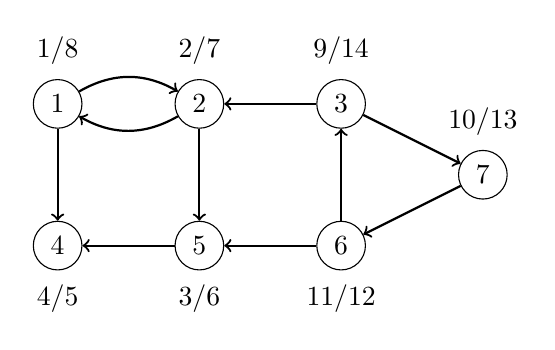
\begin{tikzpicture}[scale=0.9,label distance=-2mm]
\node[draw, circle] (1) at (-1,1) {$7$};
\node[draw, circle] (2) at (-3,2) {$3$};
\node[draw, circle] (4) at (-5,2) {$2$};
\node[draw, circle] (6) at (-7,2) {$1$};
\node[draw, circle] (3) at (-3,0) {$6$};
\node[draw, circle] (5) at (-5,0) {$5$};
\node[draw, circle] (7) at (-7,0) {$4$};

\node at (-7,2.75) {$1/8$};
\node at (-5,2.75) {$2/7$};
\node at (-3,2.75) {$9/14$};
\node at (-7,-0.75) {$4/5$};
\node at (-5,-0.75) {$3/6$};
\node at (-3,-0.75) {$11/12$};
\node at (-1,1.75) {$10/13$};

\path[draw,thick,->] (2) -- (1);
\path[draw,thick,->] (1) -- (3);
\path[draw,thick,->] (3) -- (2);
\path[draw,thick,->] (2) -- (4);
\path[draw,thick,->] (3) -- (5);
\path[draw,thick,->] (4) edge [bend left] (6);
\path[draw,thick,->] (6) edge [bend left] (4);
\path[draw,thick,->] (4) -- (5);
\path[draw,thick,->] (5) -- (7);
\path[draw,thick,->] (6) -- (7);
\end{tikzpicture}
\end{center}

Ký hiệu $x/y$ có nghĩa là
việc xử lý nút bắt đầu
tại thời điểm $x$ và kết thúc tại thời điểm $y$.
Do đó, danh sách tương ứng như sau:

\begin{tabular}{ll}
\\
nút & thời gian xử lý xong \\
\hline
4 & 5 \\
5 & 6 \\
2 & 7 \\
1 & 8 \\
6 & 12 \\
7 & 13 \\
3 & 14 \\
\\
\end{tabular}

\subsubsection{Tìm kiếm 2}

Giai đoạn thứ hai của thuật toán
hình thành các thành phần liên thông mạnh
của đồ thị.
Đầu tiên, thuật toán đảo ngược mọi
cạnh trong đồ thị.
Điều này đảm bảo rằng trong lần tìm kiếm thứ hai,
chúng ta sẽ luôn tìm thấy các thành phần liên thông mạnh
mà không có các nút thừa.

Sau khi đảo ngược các cạnh,
đồ thị ví dụ như sau:
\begin{center}
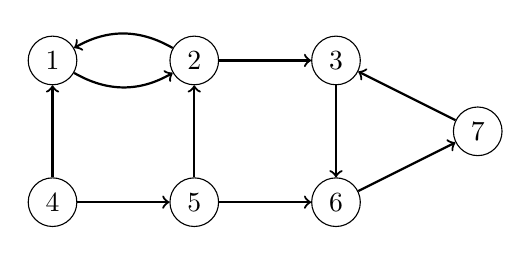
\begin{tikzpicture}[scale=0.9,label distance=-2mm]
\node[draw, circle] (1) at (-1,1) {$7$};
\node[draw, circle] (2) at (-3,2) {$3$};
\node[draw, circle] (4) at (-5,2) {$2$};
\node[draw, circle] (6) at (-7,2) {$1$};
\node[draw, circle] (3) at (-3,0) {$6$};
\node[draw, circle] (5) at (-5,0) {$5$};
\node[draw, circle] (7) at (-7,0) {$4$};

\path[draw,thick,<-] (2) -- (1);
\path[draw,thick,<-] (1) -- (3);
\path[draw,thick,<-] (3) -- (2);
\path[draw,thick,<-] (2) -- (4);
\path[draw,thick,<-] (3) -- (5);
\path[draw,thick,<-] (4) edge [bend left] (6);
\path[draw,thick,<-] (6) edge [bend left] (4);
\path[draw,thick,<-] (4) -- (5);
\path[draw,thick,<-] (5) -- (7);
\path[draw,thick,<-] (6) -- (7);
\end{tikzpicture}
\end{center}

Sau đó, thuật toán duyệt qua
danh sách các nút được tạo bởi lần tìm kiếm đầu tiên,
theo thứ tự \emph{ngược lại}.
Nếu một nút không thuộc về một thành phần nào,
thuật toán tạo một thành phần mới
và bắt đầu một tìm kiếm theo chiều sâu
thêm tất cả các nút mới tìm thấy trong quá trình tìm kiếm
vào thành phần mới.

Trong đồ thị ví dụ, thành phần đầu tiên
bắt đầu tại nút 3:

\begin{center}
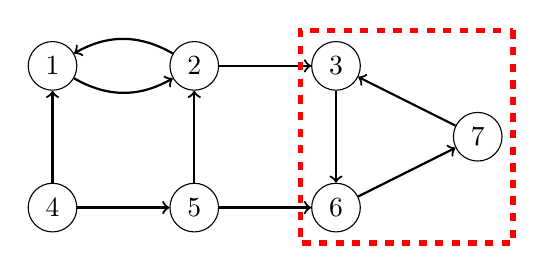
\begin{tikzpicture}[scale=0.9,label distance=-2mm]
\node[draw, circle] (1) at (-1,1) {$7$};
\node[draw, circle] (2) at (-3,2) {$3$};
\node[draw, circle] (4) at (-5,2) {$2$};
\node[draw, circle] (6) at (-7,2) {$1$};
\node[draw, circle] (3) at (-3,0) {$6$};
\node[draw, circle] (5) at (-5,0) {$5$};
\node[draw, circle] (7) at (-7,0) {$4$};

\path[draw,thick,<-] (2) -- (1);
\path[draw,thick,<-] (1) -- (3);
\path[draw,thick,<-] (3) -- (2);
\path[draw,thick,<-] (2) -- (4);
\path[draw,thick,<-] (3) -- (5);
\path[draw,thick,<-] (4) edge [bend left] (6);
\path[draw,thick,<-] (6) edge [bend left] (4);
\path[draw,thick,<-] (4) -- (5);
\path[draw,thick,<-] (5) -- (7);
\path[draw,thick,<-] (6) -- (7);

\draw [red,thick,dashed,line width=2pt] (-0.5,2.5) rectangle (-3.5,-0.5);
\end{tikzpicture}
\end{center}

Lưu ý rằng vì tất cả các cạnh đều bị đảo ngược,
thành phần không bị "tràn" sang các phần khác trong đồ thị.

\begin{samepage}
Các nút tiếp theo trong danh sách là nút 7 và 6,
nhưng chúng đã thuộc về một thành phần,
vì vậy thành phần mới tiếp theo bắt đầu tại nút 1:

\begin{center}
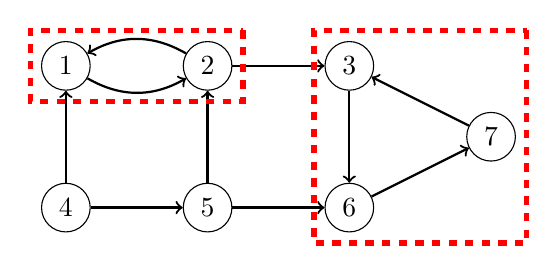
\begin{tikzpicture}[scale=0.9,label distance=-2mm]
\node[draw, circle] (1) at (-1,1) {$7$};
\node[draw, circle] (2) at (-3,2) {$3$};
\node[draw, circle] (4) at (-5,2) {$2$};
\node[draw, circle] (6) at (-7,2) {$1$};
\node[draw, circle] (3) at (-3,0) {$6$};
\node[draw, circle] (5) at (-5,0) {$5$};
\node[draw, circle] (7) at (-7,0) {$4$};

\path[draw,thick,<-] (2) -- (1);
\path[draw,thick,<-] (1) -- (3);
\path[draw,thick,<-] (3) -- (2);
\path[draw,thick,<-] (2) -- (4);
\path[draw,thick,<-] (3) -- (5);
\path[draw,thick,<-] (4) edge [bend left] (6);
\path[draw,thick,<-] (6) edge [bend left] (4);
\path[draw,thick,<-] (4) -- (5);
\path[draw,thick,<-] (5) -- (7);
\path[draw,thick,<-] (6) -- (7);

\draw [red,thick,dashed,line width=2pt] (-0.5,2.5) rectangle (-3.5,-0.5);
\draw [red,thick,dashed,line width=2pt] (-4.5,2.5) rectangle (-7.5,1.5);
%\draw [red,thick,dashed,line width=2pt] (-4.5,0.5) rectangle (-5.5,-0.5);
%\draw [red,thick,dashed,line width=2pt] (-6.5,0.5) rectangle (-7.5,-0.5);
\end{tikzpicture}
\end{center}
\end{samepage}

\begin{samepage}
Cuối cùng, thuật toán xử lý các nút 5 và 4
tạo ra các thành phần liên thông mạnh còn lại:

\begin{center}
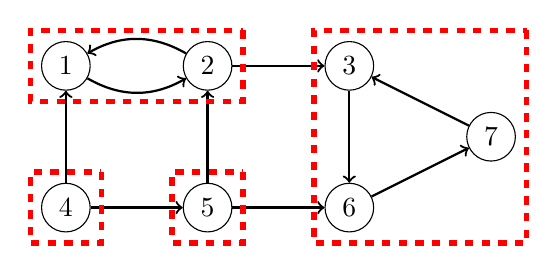
\begin{tikzpicture}[scale=0.9,label distance=-2mm]
\node[draw, circle] (1) at (-1,1) {$7$};
\node[draw, circle] (2) at (-3,2) {$3$};
\node[draw, circle] (4) at (-5,2) {$2$};
\node[draw, circle] (6) at (-7,2) {$1$};
\node[draw, circle] (3) at (-3,0) {$6$};
\node[draw, circle] (5) at (-5,0) {$5$};
\node[draw, circle] (7) at (-7,0) {$4$};

\path[draw,thick,<-] (2) -- (1);
\path[draw,thick,<-] (1) -- (3);
\path[draw,thick,<-] (3) -- (2);
\path[draw,thick,<-] (2) -- (4);
\path[draw,thick,<-] (3) -- (5);
\path[draw,thick,<-] (4) edge [bend left] (6);
\path[draw,thick,<-] (6) edge [bend left] (4);
\path[draw,thick,<-] (4) -- (5);
\path[draw,thick,<-] (5) -- (7);
\path[draw,thick,<-] (6) -- (7);

\draw [red,thick,dashed,line width=2pt] (-0.5,2.5) rectangle (-3.5,-0.5);
\draw [red,thick,dashed,line width=2pt] (-4.5,2.5) rectangle (-7.5,1.5);
\draw [red,thick,dashed,line width=2pt] (-4.5,0.5) rectangle (-5.5,-0.5);
\draw [red,thick,dashed,line width=2pt] (-6.5,0.5) rectangle (-7.5,-0.5);
\end{tikzpicture}
\end{center}
\end{samepage}

Độ phức tạp thời gian của thuật toán là $O(n+m)$,
bởi vì thuật toán
thực hiện hai lần tìm kiếm theo chiều sâu.

\section{Bài toán 2SAT}

\index{2SAT problem}

Liên thông mạnh cũng liên quan đến
\key{bài toán 2SAT (2SAT problem)}\footnote{Thuật toán được trình bày ở đây đã được
giới thiệu trong \cite{asp79}.
Cũng có một thuật toán thời gian tuyến tính nổi tiếng khác \cite{eve75}
dựa trên quay lui (backtracking).}.
Trong bài toán này, chúng ta được cho một công thức logic
\[
(a_1 \lor b_1) \land (a_2 \lor b_2) \land \cdots \land (a_m \lor b_m),
\]
trong đó mỗi $a_i$ và $b_i$ là một biến logic
($x_1,x_2,\ldots,x_n$)
hoặc là phủ định của một biến logic
($\lnot x_1, \lnot x_2, \ldots, \lnot x_n$).
Các ký hiệu ''$\land$'' và ''$\lor$'' biểu thị
các toán tử logic ''và'' và ''hoặc''.
Nhiệm vụ của chúng ta là gán cho mỗi biến một giá trị
sao cho công thức là đúng, hoặc phát biểu
rằng điều này là không thể.

Ví dụ, công thức
\[
L_1 = (x_2 \lor \lnot x_1) \land
      (\lnot x_1 \lor \lnot x_2) \land
      (x_1 \lor x_3) \land
      (\lnot x_2 \lor \lnot x_3) \land
      (x_1 \lor x_4)
\]
là đúng khi các biến được gán như sau:

\[
\begin{cases}
x_1 = \textrm{false} \\
x_2 = \textrm{false} \\
x_3 = \textrm{true} \\
x_4 = \textrm{true} \\
\end{cases}
\]

Tuy nhiên, công thức
\[
L_2 = (x_1 \lor x_2) \land
      (x_1 \lor \lnot x_2) \land
      (\lnot x_1 \lor x_3) \land
      (\lnot x_1 \lor \lnot x_3)
\]
luôn sai, bất kể chúng ta
gán giá trị như thế nào.
Lý do cho điều này là chúng ta không thể
chọn một giá trị cho $x_1$
mà không tạo ra mâu thuẫn.
Nếu $x_1$ là sai, cả $x_2$ và $\lnot x_2$
phải là đúng, điều này là không thể,
và nếu $x_1$ là đúng, cả $x_3$ và $\lnot x_3$
phải là đúng, điều này cũng không thể.

Bài toán 2SAT có thể được biểu diễn dưới dạng một đồ thị
có các nút tương ứng với
các biến $x_i$ và các phủ định $\lnot x_i$,
và các cạnh xác định các mối liên kết
giữa các biến.
Mỗi cặp $(a_i \lor b_i)$ tạo ra hai cạnh:
$\lnot a_i \to b_i$ và $\lnot b_i \to a_i$.
Điều này có nghĩa là nếu $a_i$ không đúng,
thì $b_i$ phải đúng, và ngược lại.

Đồ thị cho công thức $L_1$ là:
\\
\begin{center}
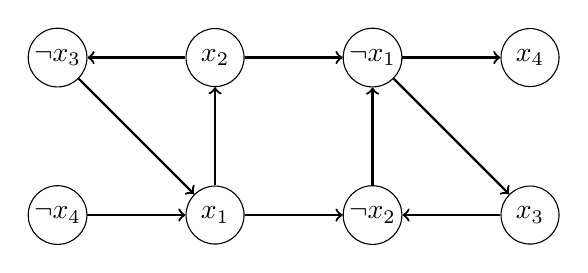
\begin{tikzpicture}[scale=1.0,minimum size=2pt]
\node[draw, circle, inner sep=1.3pt] (1) at (1,2) {$\lnot x_3$};
\node[draw, circle] (2) at (3,2) {$x_2$};
\node[draw, circle, inner sep=1.3pt] (3) at (1,0) {$\lnot x_4$};
\node[draw, circle] (4) at (3,0) {$x_1$};
\node[draw, circle, inner sep=1.3pt] (5) at (5,2) {$\lnot x_1$};
\node[draw, circle] (6) at (7,2) {$x_4$};
\node[draw, circle, inner sep=1.3pt] (7) at (5,0) {$\lnot x_2$};
\node[draw, circle] (8) at (7,0) {$x_3$};
 
\path[draw,thick,->] (1) -- (4);
\path[draw,thick,->] (4) -- (2);
\path[draw,thick,->] (2) -- (1);
\path[draw,thick,->] (3) -- (4);
\path[draw,thick,->] (2) -- (5);
\path[draw,thick,->] (4) -- (7);
\path[draw,thick,->] (5) -- (6);
\path[draw,thick,->] (5) -- (8);
\path[draw,thick,->] (8) -- (7);
\path[draw,thick,->] (7) -- (5);
\end{tikzpicture}
\end{center}
Và đồ thị cho công thức $L_2$ là:
\\
\begin{center}
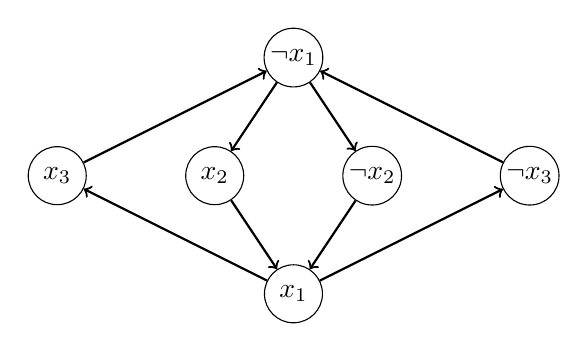
\begin{tikzpicture}[scale=1.0,minimum size=2pt]
\node[draw, circle] (1) at (1,2) {$x_3$};
\node[draw, circle] (2) at (3,2) {$x_2$};
\node[draw, circle, inner sep=1.3pt] (3) at (5,2) {$\lnot x_2$};
\node[draw, circle, inner sep=1.3pt] (4) at (7,2) {$\lnot x_3$};
\node[draw, circle, inner sep=1.3pt] (5) at (4,3.5) {$\lnot x_1$};
\node[draw, circle] (6) at (4,0.5) {$x_1$};

\path[draw,thick,->] (1) -- (5);
\path[draw,thick,->] (4) -- (5);
\path[draw,thick,->] (6) -- (1);
\path[draw,thick,->] (6) -- (4);
\path[draw,thick,->] (5) -- (2);
\path[draw,thick,->] (5) -- (3);
\path[draw,thick,->] (2) -- (6);
\path[draw,thick,->] (3) -- (6);
\end{tikzpicture}
\end{center}

Cấu trúc của đồ thị cho chúng ta biết liệu
có thể gán các giá trị
của các biến sao cho
công thức là đúng hay không.
Hóa ra điều này có thể được thực hiện
chính xác khi không có các nút
$x_i$ và $\lnot x_i$ nào mà
cả hai nút đều thuộc về
cùng một thành phần liên thông mạnh.
Nếu có các nút như vậy,
đồ thị chứa
một đường đi từ $x_i$ đến $\lnot x_i$
và cũng có một đường đi từ $\lnot x_i$ đến $x_i$,
vì vậy cả $x_i$ và $\lnot x_i$ đều phải là đúng
điều này là không thể.

Trong đồ thị của công thức $L_1$
không có các nút $x_i$ và $\lnot x_i$ nào
mà cả hai nút
đều thuộc cùng một thành phần liên thông mạnh,
vì vậy một lời giải tồn tại.
Trong đồ thị của công thức $L_2$
tất cả các nút đều thuộc cùng một thành phần liên thông mạnh,
vì vậy một lời giải không tồn tại.

Nếu một lời giải tồn tại, các giá trị cho các biến
có thể được tìm thấy bằng cách duyệt qua các nút của
đồ thị thành phần theo thứ tự sắp xếp tô pô ngược.
Tại mỗi bước, chúng ta xử lý một thành phần
không chứa các cạnh dẫn đến một
thành phần chưa được xử lý.
Nếu các biến trong thành phần
chưa được gán giá trị,
giá trị của chúng sẽ được xác định
theo các giá trị trong thành phần,
và nếu chúng đã có giá trị,
chúng vẫn không thay đổi.
Quá trình tiếp tục cho đến khi mỗi biến
đã được gán một giá trị.

Đồ thị thành phần cho công thức $L_1$ như sau:
\begin{center}
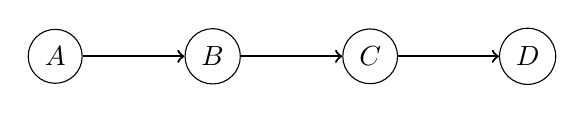
\begin{tikzpicture}[scale=1.0]
\node[draw, circle] (1) at (0,0) {$A$};
\node[draw, circle] (2) at (2,0) {$B$};
\node[draw, circle] (3) at (4,0) {$C$};
\node[draw, circle] (4) at (6,0) {$D$};

\path[draw,thick,->] (1) -- (2);
\path[draw,thick,->] (2) -- (3);
\path[draw,thick,->] (3) -- (4);
\end{tikzpicture}
\end{center}

Các thành phần là
$A = \{\lnot x_4\}$,
$B = \{x_1, x_2, \lnot x_3\}$,
$C = \{\lnot x_1, \lnot x_2, x_3\}$ và
$D = \{x_4\}$.
Khi xây dựng lời giải,
chúng ta trước tiên xử lý thành phần $D$
nơi $x_4$ trở thành đúng.
Sau đó, chúng ta xử lý thành phần $C$
nơi $x_1$ và $x_2$ trở thành sai
và $x_3$ trở thành đúng.
Tất cả các biến đã được gán giá trị,
vì vậy các thành phần còn lại $A$ và $B$
không thay đổi các biến.

Lưu ý rằng phương pháp này hoạt động, bởi vì
đồ thị có một cấu trúc đặc biệt:
nếu có các đường đi từ nút $x_i$ đến nút $x_j$
và từ nút $x_j$ đến nút $\lnot x_j$,
thì nút $x_i$ không bao giờ trở thành đúng.
Lý do cho điều này là cũng có
một đường đi từ nút $\lnot x_j$ đến nút $\lnot x_i$,
và cả $x_i$ và $x_j$ đều trở thành sai.

\index{3SAT problem}

Một bài toán khó hơn là \key{bài toán 3SAT (3SAT problem)},
trong đó mỗi phần của công thức có dạng
$(a_i \lor b_i \lor c_i)$.
Bài toán này là NP-khó (NP-hard), vì vậy không có thuật toán hiệu quả nào
được biết đến để giải quyết bài toán này.